% Copyright 2010, Piotr Jakubowski

\chapter{Introduction}
  \section{Problem Description}
  Along with the huge popularization of the Internet there appeared enormous market for all sorts of web applications. Every month, big companies as well as small startups try to get as much of this market, bringing in new features and shocking the crowd with innovative functionalities. Surprisingly, the market seems to be far from saturation, as brilliant ideas except for fulfilling known demand create new needs as well.

  New tools started to emerge in order to meet the needs of Internet population. Dynamic languages started to supersede old and known. Python and Ruby became the new Java and C. The speed of development surpassed the speed of execution, as technical limitations and price of servers are not the issue any more. Moreover, web development frameworks made it possible to code the application on the new level of abstraction - we can instantaneously start to implement our business logic, without the need to think about how we should persist our business models into database and how we should handle requests and respond to them. Java developers got Spring and Hibernate, but the noteworthy Ruby on Rails took web development to the whole new level as mentioned before. The threshold of making the ideas happen has been successfully shrunken.
  
  As mentioned before, today's software development has been focused on the effectiveness and speed of development. A lot of work has been done to create developer-oriented tools that try to make developing business ideas effortless.
  
  Of course, there is plenty of room for improvements. One of them is the idea of automating process of creating the administration panel for the application. Very often administration part of the application is mundane part of CRUD\footnote{Create Read Update Delete} actions. It is the "must do" part. 
  
   User-oriented features is the target thing of development. This is what makes money and keeps us all employed. It seems like possibility to be able to automatically generate panel for administering our resources would make development of web application even more dynamic. It would bring plenty of benefits, such as:
  
  \begin{itemize}
	  \item Whole team can focus on what really matters, which is creating functionality that would be an added-value for our users
	  \item Creating new features and resources to our application would require less effort - as soon as we have user-oriented functionality ready the administration part is automatically generated.
	  \item Business people connected with our project can instantly browse new resources in our application.
	\end{itemize}
  
  Thereby, the aim of this thesis is to create and demonstrate the process of creation of plugin that would enable automatic generation of administration part of the application. The plugin would be developed for, mentioned before, Ruby on Rails framework.
  
  \section{Existing Solutions}
  Thanks to its rapidly growing popularity, Ruby and Ruby on Rails got very broad community. Not only does it result in a huge number of places you can ask for help, but also in all kind of libraries that would make the life of web developer easier. And as it seems I am not alone stating the problem described above. There are already several implementations that attack this problem. Some of them are more successful than others, there are different kind of approaches and different outcomes. 
  
  In order to see what market has to offer I looked through available solutions and chose 3 most popular ones in order to see what kind of functionalities they provide and what flaws they suffer from. 
  
    \subsection[Active Scaffold] {Active Scaffold\footnote{http://activescaffold.com/}}
      According to Ruby Toolbox\footnote{http://ruby-toolbox.com/categories/rails\_admin\_interfaces.html} the most popular plugin for admin interface generation. Unfortunately, it seems like the days of glory for this gem are long gone. The plugin does not support Rails in version 3, which despite being released very recently already became a standard for new applications. 
      
      Technicalities aside, it seems to be rather functional. The almost out-of-the-box look is presented on figure \ref{activescaffold1}.
      \begin{figure}[h]
    		\begin{center}
    			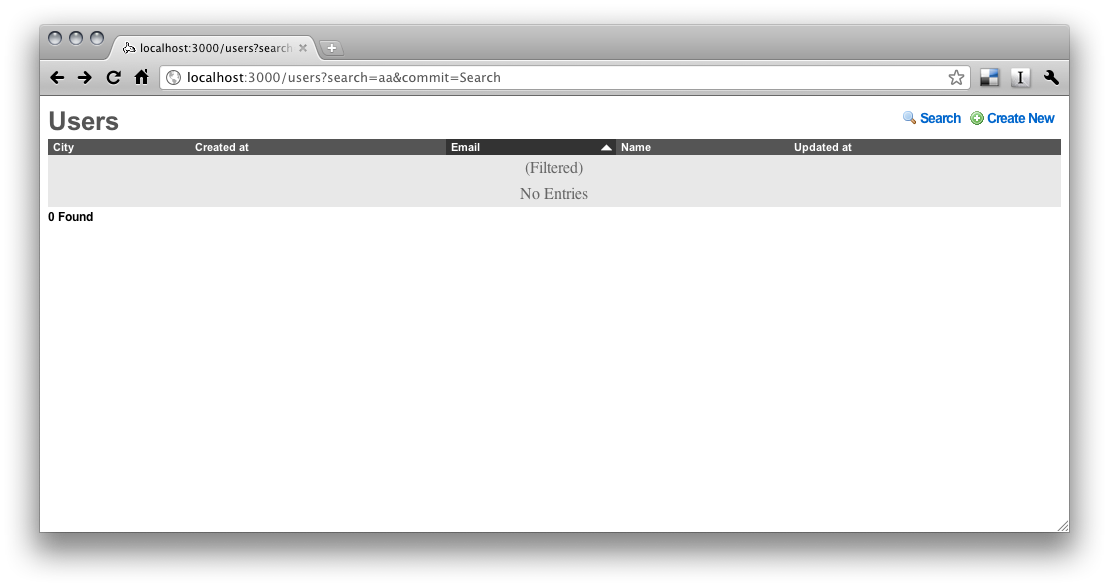
\includegraphics[width=\linewidth]{images/chapter01/activescaffold1.png}
    			\caption{Active Scaffold}
    			\label{activescaffold1}
    		\end{center}
    	\end{figure}

    \subsection{Typus}
      TBD
  
    \subsection{admin\_data}
      TBD
    
  
  
  \section{Solution Proposal}
    \subsection{Solution Proposal}
    TBD
  
    \subsection{Projected Challenges}
    TBD